%%%%%%%%%%%%%%%%%%%%%%%%%%%%%%%%%%%%%%%%%%%%%%%%%%%%%%%%%%%
%% Congratulations, you've made an excellent choice
%% of writing your Tampere University thesis using
%% the LaTeX system. This document attempts to be
%% as complete a template as possible to let you focus
%% on the most important part: the writing itself.
%% Thus the details regarding the visual appearance
%% and even structure have already been worked out
%% for you!
%%
%% I sincerely hope you will find this template useful
%% in completing your thesis project. I've tried to
%% add comments (followed by the % sign) to clarify
%% the structure and purpose of some of the commands.
%% Most of the magic happens in the file tauthesis.cls,
%% which you are more than welcome to take a look at.
%% Just refrain from editing it in the most crucial
%% versions of the thesis!
%%
%% I wish you and your thesis project the best of luck!
%% If this template causes you trouble along the way
%% or if you've any suggestions for improving it,
%% please contact me via email at
%% 
%% ville.koljonen (at) tuni.fi.
%%
%% Yours,
%%
%% Ville Koljonen
%% 16th May 2019
%%
%% PS. This template or its associated class file don't
%% come with a warranty. The content is provided as is,
%% without even the implied promise of fitness to the
%% mentioned purpose. You, as the author of the thesis,
%% are responsible for the entire work, including the
%% provided material. No one else is liable to you for
%% any damage inflicted on you or your thesis, were it
%% caused by using this template or not.
%%%%%%%%%%%%%%%%%%%%%%%%%%%%%%%%%%%%%%%%%%%%%%%%%%%%%%%%%%%

%%%%% NOTICE %%%%%
%% Please read through the entire template
%% (files under ./tex) to find all instructions.
%% It is possible that the attached pdf files
%% do not include the latest information.
%%%%%%%%%%%%%%%%%%

%%%%% INSTRUCTIONS FOR COMPILING THE DOCUMENT %%%%%
%% Overleaf: just click Recompile.
%% Terminal:
%%  1. pdflatex main.tex
%%  2. makeindex -s main.ist -t main.glg -o main.gls main.glo
%%  3. biber main
%%  4. pdflatex main.tex
%%  5. pdflatex main.tex
%% Similar sequence of commands is also required
%% in LaTeX specific editors.
%%%%%%%%%%%%%%%%%%%%%%%%%%%%%%%%%%%%%%%%%%%%%%%%%%%

%%%%% PREAMBLE %%%%%

%%%%% Document class declaration.
% The possible optional arguments are
%   finnish - thesis in Finnish (default)
%   english - thesis in English
%   numeric - citations in numeric style (default)
%   authoryear - citations in author-year style
%   apa - citations in APA 7 (available only in English)
%   ieee - citations in IEEE style
%       apa and ieee provide biblatex basic styles as is!
%   draft - for faster non-final works, also skips images
%           (recommended, remove in final version)
%   programs - if you wish to display code snippets
% Example: \documentclass[english, authoryear]{tauthesis}
%          thesis in English with author-year citations
\documentclass[english]{tauthesis}

% The glossaries package throws a warning:
% No language module detected for 'finnish'.
% You can safely ignore this. All other
% warnings should be taken care of!

%%%%% Your packages.
% Before adding packages, see if they can be found
% in tauthesis.cls already. If you're not sure that
% you need a certain package, don't include it in
% the document! This can dramatically reduce
% compilation time.

% Graphs
% \usepackage{pgfplots}
% \pgfplotsset{compat=1.15}

% Subfigures and wrapping text
% \usepackage{subcaption}

% Mathematics packages
\usepackage{amsmath, amssymb, amsthm}
%\usepackage{bm}

% Chemistry packages
% Newest mhchem is attached for compatibility
% \usepackage{chemfig}
% \usepackage[version=4]{mhchem}

% Text hyperlinking
% \usepackage{hyperref}
% \hypersetup{hidelinks}

% (SI) unit handling
% \usepackage{siunitx}

%\sisetup{
%    detect-all,
%    math-sf=\mathrm,
%    exponent-product=\cdot,
%    output-decimal-marker={,} % for theses in FINNISH!
%}

%%%%% Your commands.

% Print verbatim LaTeX commands
\newcommand{\verbcommand}[1]{\texttt{\textbackslash #1}}

% Basic theorems in Finnish and in English.
% Remove [chapter] if you wish a simply
% running enumeration.
% \newtheorem{lause}{Lause}[chapter]
% \newtheorem{theorem}[lause]{Theorem}

% \newtheorem{apulause}[lause]{Apulause}
% \newtheorem{lemma}[lause]{Lemma}

% Use these versions for individually
% enumerated lemmas
% \newtheorem{apulause}{Apulause}[chapter]
% \newtheorem{lemma}{Lemma}[chapter]

% Definition style
% \theoremstyle{definition}
% \newtheorem{maaritelma}{Määritelmä}[chapter]
% \newtheorem{definition}[maaritelma]{Definition}
% examples in this style

%%%%% Glossary information.

\loadglsentries[main]{tex/sanasto.tex}
\makeglossaries

%%%%% Citation information.

\addbibresource{tex/references.bib}

\begin{document}

%%%%% FRONT MATTER %%%%%

\frontmatter

%%%%% Thesis information and title page.

% The titles of the work. If there is no subtitle,
% leave the arguments empty. Pass the title in
% the primary language as the first argument
% and its translation to the secondary language
% as the second.
\title{Title}{Kuvaava otsikko}
\subtitle{Tarkentava alaotsikko}{A Specifying Subtitle}

% The author name.
\author{Väinö-Waltteri Granat}

% The examiner information.
% If your work has multiple examiners, replace with
% \examiner[<label>]{<name> \\ <name>}
% where <label> is an appropriate (plural) label,
% e.g. Examiners or Tarkastajat, and <name>s are
% replaced by the examiner names, each on their
% separate line.
\examiner[Examiner]{Prof. Joni Kämäräinen}

% The finishing date of the thesis (YYYY-MM-DD).
\finishdate{2020}{05}{18}

% The type of the thesis (e.g. Kandidaatintyö
% or Master of Science Thesis) in the primary
% and the secondary languages of the thesis.
\thesistype{Opinnäytetyön taso}{Thesis type}

% The faculty and degree programme names in
% the primary and the secondary languages of
% the thesis.
\facultyname{Tiedekunnan nimi}{Faculty Name}
\programmename{Tutkinto-ohjelma}{Degree Programme}

% The keywords to the thesis in the primary and
% the secondary languages of the thesis
\keywords%
    {avainsana, avainsana, avainsana, avainsana, avainsana}
    {keyword, keyword, keyword, keyword, keyword}

\maketitle

%%%%% Abstracts and preface.

% Write the abstract(s) and the preface
% into a separate file for the sake of clarity.
% Pass the appropriate file name as the first
% argument to these commands. Put the \abstract
% in the primary language first and the
% \otherabstract in the secondary language second.
% Those who do not speak Finnish only need the
% first abstract. The second argument of
% the \preface command takes the place where
% the thesis was signed in.
\abstract{tex/tiivistelma.tex}
\otherabstract{tex/abstract.tex}
\preface{tex/alkusanat.tex}{Tampereella}

%%%%% Table of contents.

\tableofcontents

%%%%% Lists of figures, tables, listings and terms.

% Print the lists of figures and/or tables.
% Uncomment either of these commands as required.
% Both are optional, but if there are many important
% figures/tables, listing them may be a good idea.

% \listoffigures
% \listoftables
% \lstlistoflistings

% Print the glossary of terms.

\glossary

%%%%% MAIN MATTER %%%%%

\mainmatter

% Write each of the chapters of the thesis
% into a separate file for the sake of clarity.
% They can be \input as shown below. Give both
% the chapters and their files as descriptive
% names as possible.
\chapter{Introduction}
\label{ch:johdanto}
Speech is the most important form of human communication. This is why it's not
suprising that humans have been developing machines to produce artificial speech
as far back as 18th century~\cite{SchroederManfredR1993Abho}. Such machines
allow communication in situations where one of the participants is not
able to produce audible speech for the rest. This might be because of physical
distance, physiolocigal inability or the speaker might not be a human in the
first place. Modern artificial speech solutions are most often created as
computer programs called text to speech applications. 

% Is physiolocigal inability appropriate phrase
% Check if TTS applications is right


This study is done in concurrency to a larger project of
deep speaking avatar which seeks to create a human like digital avatar, that anyone
can interact with by speaking to. Goal of this study is to produce a
text to speech system for that avatar by using state of the art deep learning
methods. The system implements a pretrained text to speech neural network called
Tacotron2~\cite{shen2018natural}.

The structure of this thesis is as follows. 

\chapter{Esitystyyli}
\label{ch:esitystyyli}
Tekstin sisällön lisäksi esitystyyli vaikuttaa suuresti viestinnän onnistumiseen. Ulkoasu ja kirjoitustyyli antavat työstä ja kirjoittajasta kuvan, toivottavasti hyvän.

\section{Teksti}

Älä suotta murehdi tekstin asettelusta, tämä pohja hoitaa sen jo valmiiksi. Kirjoitustyylin perusohjeet ovat:

\begin{itemize}
\item Ajattele lukijaa aina tekstiä kirjoittaessasi ja johdattele häntä riittävästi. Anna ensin yleiskuva ja liitä siihen yksityiskohdat. 
\item Korosta tärkeimmät asiat, esimerkiksi nostamalla ne omiksi luvuikseen (\verbcommand{section}, \verbcommand{subsection}), poimimalla taulukkoon tai selittämällä kuvan avulla. Tekstissä käytä korostamiseen kursivointia (\verbcommand{emph}), mutta älä korosta liikaa.
\item Vältä pitkiä virkkeitä ja monimutkaisia lauserakenteita. Piste on paras välimerkki. 
\item Suosi aktiivimuodossa olevia verbejä ja sijoita ne lauseen alkupuolelle. Älä kuitenkaan käytä yksikön 1. persoonaa (minä) kuin alkusanoissa. 
\item Vältä kapulakielisiä ilmauksia ja ammattislangia. Sano asiat suoraan. Käytä vakiintunutta teknistä sanastoa, merkintöjä ja neutraalia asiatyyliä. 
\item Lukujen ja alalukujen tulee olla vähintään kahden kappaleen mittaisia ja mielellään keskenään tasapainoisia. Kappale muodostuu aina useammasta kuin yhdestä virkkeestä. 
\item Luvut ja alaluvut numeroidaan korkeintaan kolmannelle tasolle (\verbcommand{subsection}) asti, esimerkiksi 4.4.2. Pohja huolehtii tästäkin automaattisesti.
\item Lyhenteitä ei tulisi käyttää liikaa. Käytä lyhenteissä pieniä ja isoja kirjaimia johdonmukaisesti. 
\end{itemize}

\section{Kuvat}

Kaikkiin kuviin täytyy viitata tekstissä. Kuvan avulla voidaan esittää tietoa tiiviissä muodossa, mutta kuvan täytyy olla merkityksellinen työn sisällön kannalta ja kuva täytyy selittää tekstissä. Viittaus on mielellään samalla sivulla kuin kuva tai sitä ennen. Kuvat ja taulukot numeroidaan ja sijoitetaan pääsääntöisesti sivun yläreunaan, oman harkinnan mukaan. \LaTeX{}issa tämä tapahtuu sijoittamalla \verbcommand{caption}-komentoa seuraavalle riville \verbcommand{label}-komennon, jonka argumentti on kyseisen kuvan (tai taulukon) yksikäsitteinen tunniste. Viittaaminen tapahtuu \verbcommand{ref}-komennolla, johon syötetään haluttu tunniste. Lukua ei saa aloittaa (eikä mielellään lopettaa) kuvalla, taulukolla, kaavalla tai luettelolla, vaan sen ympärillä on oltava tekstiä. Kuvateksti sijoitetaan kuvan alle.

Kuvan keskeinen sisältö on selitettävä tekstissä, jotta sen sanomasta ei jää epäselvyyttä. Analysointiohjelmistojen tuottamat kuvat vaativat useimmiten muokkausta, kuten kuvassa \ref{fig:huolittelu}. Kuvan tekstien on oltava luettavissa, ja niiden kooksi suositellaan samaa kuin muussa tekstissä, 11 pt. Pyri siihen, että myös harmaasävyissä tulostettu kopio on luettava ja selkeä. Suosi vektorimuotoisia kuvatiedostotyyppejä \texttt{.eps} ja \texttt{.pdf} (\LaTeX{} ei syö \texttt{.svg}-tiedostoja\ldots), sillä niitä voi skaalata helposti laadun heikkenemättä. \LaTeX{} sisältää myös erittäin ilmaisuvoimaisia paketteja vektorigrafiikan (\texttt{tikz}) \parencite{tikz} ja kuvaajien (\texttt{pgfplots}) \parencite{pgfplots} piirtämiseen. Kuvassa \ref{fig:pgf-esimerkki} esitetään esimerkki jälkimmäisen avulla luodusta kuvaajasta.

\begin{figure}
\centering
%\begin{subfigure}{0.49\textwidth}
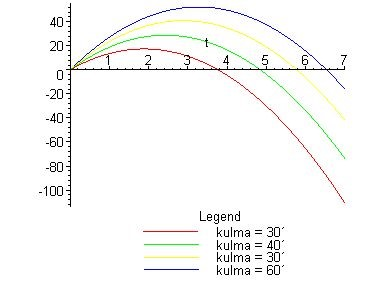
\includegraphics[width=\textwidth]{figures/bad-example.jpg}
%\end{subfigure}
%\begin{subfigure}{0.49\textwidth}
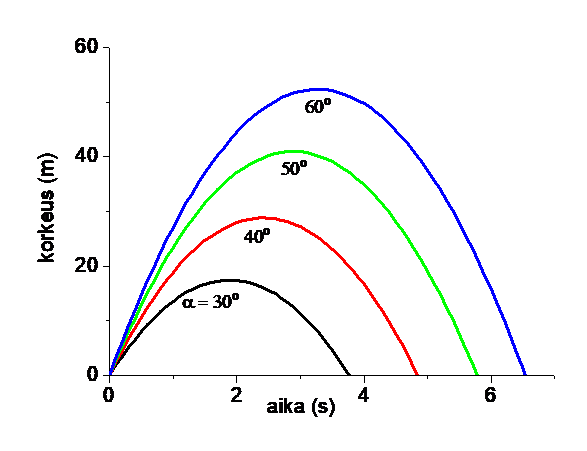
\includegraphics[width=\textwidth]{figures/good-example.png}
%\end{subfigure}
\caption[Tämä on lyhyt kuvateksti.]{Kuvaaja on hyvä muokata julkaisukelpoiseksi. Vasemmalla on esitetty muokkaamaton kuvaaja ja oikealla muokattu.}
\label{fig:huolittelu}
\end{figure}

\begin{figure}
\centering
%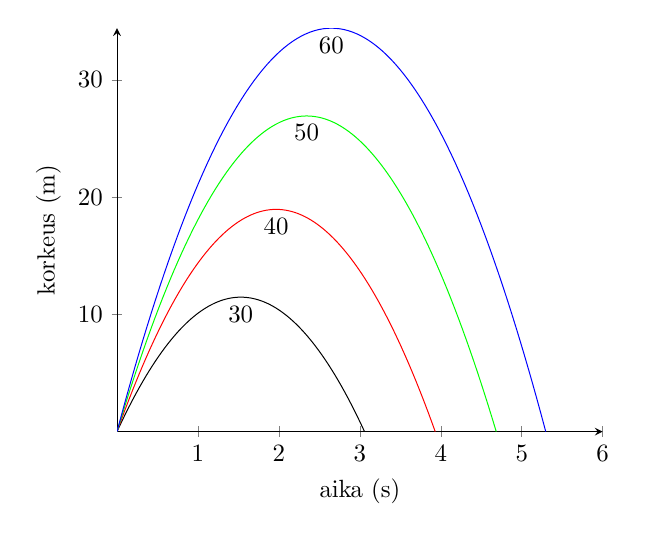
\begin{tikzpicture}[scale=0.9]
\begin{axis}[axis lines=center,
            xlabel={aika (s)},
            xlabel near ticks,
            ylabel={korkeus (m)},
            ylabel near ticks,
            xmin=0, xmax=6, ymin=0]
\addplot[color=black,
        domain=0:30*sin(30)/(0.5*9.81),
        samples=101]
        {30*sin(30)*x - 0.5*9.81*x^2}
        node[color=black, midway, below]{\ang{30}};
\addplot[color=red,
        domain=0:30*sin(40)/(0.5*9.81),
        samples=101]
        {30*sin(40)*x - 0.5*9.81*x^2}
        node[color=black, midway, below]{\ang{40}};
\addplot[color=green,
        domain=0:30*sin(50)/(0.5*9.81),
        samples=101]
        {30*sin(50)*x - 0.5*9.81*x^2}
        node[color=black, midway, below]{\ang{50}};
\addplot[color=blue,
        domain=0:30*sin(60)/(0.5*9.81),
        samples=101]
        {30*sin(60)*x - 0.5*9.81*x^2}
        node[color=black, midway, below]{\ang{60}};
\end{axis}
\end{tikzpicture}
\caption{Kuvan \ref{fig:huolittelu} tyylinen esimerkki \texttt{pgfplots}-paketilla piirrettynä.}
\label{fig:pgf-esimerkki}
\end{figure}

\section{Taulukot}

Taulukot sopivat hyvin erityisesti numeerisen informaation esittämiseen tiiviissä muodossa. Kuvien tapaan taulukot numeroidaan ja varustetaan otsikolla, kuten taulukossa. Taulukkoteksti sijoitetaan samalle sivulle taulukon kanssa ja taulukon yläpuolelle. Suureet, lyhenteet ja symbolit selitetään tarvittaessa tekstissä. Kaikkiin taulukoihin on viitattava tekstissä, mieluummin ennen taulukkoa. Taulukon keskeinen sanoma ja tulkintaohjeet selitetään tekstissä.

Taulukon sarakkeet otsikoidaan, ja suureet sekä yksiköt laitetaan näkyviin. Jos otsikkoriviä tarvitsee erottaa muusta taulukosta, tee se korostamalla (\verbcommand{emph}). Taulukon järjestyksellä on suuri merkitys. Jokaista solua ei pidä ympäröidä reunaviivalla, koska taulukosta tulee raskaslukuinen. Lisää vaakaviiva taulukon ylä- ja alareunaan. Vaakaviivoja voi käyttää esimerkiksi 4--5 rivin välein, ellei tietoja muuten ole jaettu kategorioihin tai selkeys sitä vaadi. Sarakkeen numeroarvot tasataan desimaalipilkun kohdalta, jolloin arvoja on helppo vertailla. Tämä tapahtuu \LaTeX{}issa helposti \texttt{siunitx}-paketin \parencite{siunitx} taulukkomateriaalin avulla. Tavoitteena on, että suureet ilmaistaan SI-yksikössä ja käytetään joko vakiintuneita etuliitteitä tai kymmenen potenssin muotoja siten, että ne voidaan laittaa otsikkoriville (katso tässäkin \texttt{siunitx}). Muutamia suosituksia taulukoiden ja kuvien käytöstä löydät lähteestä \parencite{pubadvice2009}.

\begin{table}
\centering
\caption{Esimerkki höyrystysolosuhteista kahdessa ohutkalvorakenteessa.}
\label{tab:taulukkoesimerkki}
% Making scarce use of table lines is recommended
% for clarity. Even the outer lines are generally
% not needed! Use the siunitx package provided
% S column type for easy decimal alignment.
%\begin{tabular}{c|S[table-format=3.1] S[table-format=1.2] S[table-format=2.1e-1] S[table-format=2.1] S[table-format=2.0]@{--}S[table-format=3.0] S[table-format=1.1]}
%    \hline
%    aine & {paksuus} & {korjauskerroin} & {paine} & {lämpötila} & \multicolumn{2}{c}{virta} & {nopeus} \\[-0.5ex]
    % The syntax \\[<length>] inserts a vertical
    % space of <length> in addition to the normal
    % new line action provided by \\. This should
    % apply in any situation.
%    & {(\si{\nano\metre})} & & {(\si{\milli\bar})} & {(\si{\degreeCelsius})} & \multicolumn{2}{c}{(\si{\milli\ampere})} & {(\si{\nano\metre\per\second})} \\\hline
%    SiO2 & 181.0 & 1.10 & 3.0e-5 & 90.6 & 20 & 23 & 0.2 \\
%    TiO2 & 122.1 & 1.55 & 15.0e-5 & 91.1 & 93 & 100 & 0.1 \\\hline
%\end{tabular}
\end{table}

\section{Matemaattiset merkinnät ja yhtälöt}

Käytä selvyyssyistä mieluummin numeroita kuin kirjaimia lukuarvoissa: esimerkiksi ''6 työvaihetta'' on selkeämpi ja parempi kuin ''kuusi työvaihetta''. Tuhaterottimen käyttö selkeyttää tekstiä, eli kirjoita 55~700~125 muodon 55700125 sijaan. Desimaalipilkkua edeltävä nolla tulee aina merkitä. Suomen kielessä käytetään virallisesti desimaalipilkkua, englannin kielessä desimaalipistettä. Näistäkin tämä pohja ja \texttt{siunitx} \parencite{siunitx} huolehtivat siististi, jos vain annat niiden (muista ottaa \texttt{siunitx} käyttöön).

Numeroiden tavoin myös mittayksiköt kannattaa kirjoittaa lyhenteinä. Mittayksikön ja numeroarvon välissä on itse asiassa välilyöntiä lyhyempi väli, ja niiden tulee olla samalla rivillä. Taulukko tai kaavio on parempi esitystapa, jos tekstin sekaan tulee runsaasti numeroarvoja. Usein numeroarvoihin voi liittää laadullisen määreen, ja vastaavasti kaikkiin laadullisiin määreisiin (suuri, pieni, kallis, nopea) tulisi liittää numeroarvo kuvaamaan suuruusluokkaa. Numeroiden kanssa ei tarvitse käyttää sijapäätettä, jos seuraava sana on samassa sijassa (taivutusmuodossa), esimerkiksi ''jakautuu 10 osaan'' ja ''20 ja 50 sentin kolikot''. On myös tapauksia, joissa sijapääte pitää merkitä, esimerkiksi lauseessa ''osallistujia oli 7:stä eri maasta''.

Tekstissä tulee ensisijaisesti käyttää yleisesti tunnettuja ja hyvin määriteltyjä käsitteitä, joiden kirjoittamiseen on yleensä jokin vakiintunut merkintätapa tai symboli. Uudet käsitteet ja merkinnät pitää määritellä, kun ne esiintyvät tekstissä ensimmäisen kerran. Symboleissa ja mittayksiköissä isot ja pienet kirjaimet tarkoittavat eri asioita. Samaa symbolia ei tule käyttää monessa eri merkityksessä. Mittayksiköt merkitään selvästi.

Matemaattiset merkit ja kreikkalaiset kirjaimet löytyvät \LaTeX{}in makroista ja kaavamoodeista, kuten $\Theta(n^2)$. Yksinkertaiset kaavat voivat olla osa virkettä (siis tekstiä) ja ilman numeroa. Esimerkkinä tekstistä erotetusta kaavasta Newtonin 2. peruslaki voidaan ilmaista muodossa
\begin{equation}\label{eq:newton2}
    m\mathbf{a} = \mathbf{F},
\end{equation}
missä $m$ on kappaleen massa, $\mathbf{a}$ sen kiihtyvyys ja $\mathbf{F}$ siihen kohdistuva nettovoima. Huomaa, että symbolien merkitys selitetään aina heti kaavan yhteydessä sillä tavalla kuin on luontevinta. Kaavat esitetään tarkoituksella eri fontilla ja matemaattiset symbolit pääosin kursivoidaan. Vektorit voidaan esittää lihavoituna, kuten edellä (tavallisinta painetussa tekstissä) tai nuolella varustettuna, kuten $\vec{v}$. Dimensiollisia lukuja voidaan esittää \verbcommand{SI}-komennon avulla:
%\begin{equation*}
%    \Vert\mathbf{F}\Vert = m\Vert\mathbf{a}\Vert = \SI{10}{\kilogram} \cdot \SI{9.81}{\metre\per\second\squared} = \SI{98.1}{\newton}.
%\end{equation*}

Matemaattinen kaava numeroidaan, jos se on omalla rivillään ja siihen viitataan muualla teks-tissä, katso esimerkiksi kaava \eqref{eq:newton2}. Usein numero on tavallisten sulkujen sisällä ja tasattu oikeaan laitaan, kuten tässä ohjeessa. Matematiikan kirjoitusohjeiden ja englatilaisen kulttuuripiirin tavan mukaisesti kaavoihin sisällytetään välimerkit, kuten yhtälössä \eqref{eq:newton2} lopun pilkku. Toisinaan matemaattisen rakenteen edessä on tunniste, kuten Määritelmä 1 tai Lause 1 \parencite{matohje2009}. Nämä luodaan omilla \texttt{amsthm}-pakettiin pohjautuvilla ympäristöillään. Kaavojen ja muiden rakenteiden numerointi voi olla juokseva läpi koko tekstin ((1), (2), \ldots) tai aina yhden luvun sisällä ((1.1), (1.2), \ldots, (2.1), \ldots).

Älä aloita uutta virkettä matemaattisella symbolilla. Yleensä teknis-fysikaalisessa tekstissä kursivoidaan muuttujat, kuten $x$ ja $y$. Kursivoinneissa luottaa \LaTeX{}in automatiikkaan \parencite{notsoshort}. Sen sijaan alkeisfunktioita, erikoisfunktioita ja operaattoreita merkitään tavallisella kirjasimella: $\sin(2x + y)$ tai
%\begin{equation*}
%    \lim_{x \rightarrow -1}\frac{x^2 - 1}{x + 1} = -2.
%\end{equation*}
Kappaletta, tai varsinkaan lukua ei ole hyvä myöskään lopettaa kaavaan, kuvaan tai taulukkoon.

%Kemian symboleita tarvitseviakaan \LaTeX{} ei jätä pulaan. Molekyylikaavoja ja reaktioyhtälöitä, kuten \ce{CH3CH2CH2COOH} ja
%\begin{center}
%    \ce{N2 (g) + 3 H2 (g) <=> 2 NH3 (g)}
%\end{center}
%varten tarvitaan \texttt{mhchem}-paketti \parencite{mhchem}, ja kokonaisia rakennekaavoja varten \texttt{chemfig} \parencite{chemfig}. Esimerkkinä jälkimmäisestä voidaan esittää telluriumtetrafluoridin (\ce{TeF4}) Lewisin rakenne.
%\begin{center}
%    \chemfig{\lewis{0:,Te}
%    (-[:90]\lewis{0:2:4:,F})
%    (-[:270]\lewis{0:4:6:,F})
%    (<:[:135]\lewis{1:3:5:,F})
%    (<[:225]\lewis{3:5:7:,F})
%    }
%\end{center}
%Varsinkin rakennekaavojen latominen vaatii totuttelemista, mutta keinot ovat olemassa.

\section{Ohjelmat ja algoritmit}

Koodin kirjasinlajina käytetään \texttt{tasalevyistä kirjasinlajia}, jonka merkit ovat yhtä leveitä. Kun ohjelmakoodin tai algoritmin pituus on alle 10 riviä eikä siihen enää myöhemmin tekstissä viitata, se voidaan esittää kuten kaavat. Pidemmät, alle sivun mittaiset ohjelmakoodit tai algoritmit kirjoitetaan kuten Ohjelma \ref{prog:esimerkki}, otsikkona ''Ohjelma'' tai ''Algoritmi''.

Koodiin on hyvä lisätä muutamia kommentteja ja sisentää se johdonmukaisesti. Koodin toiminta selitetään aina myös juoksevassa tekstissä pääpiirteissään, lähinnä siitä esitetään muutamia avainhuomioita. Esimerkiksi \LaTeX{}in paketti \texttt{listings} \parencite{listings,notsoshort} osaa kätevästi sisällyttää sekä oikeita kooditiedostoja että pseudokoodia tekstiin, lisätä automaattisesti rivinumeroinnin ja korostaa monet varatut sanat. Käytä sitä kaiken koodin esittämiseen \LaTeX{}in avulla.

% \renewcommand{\lstlistingname}{Ohjelma}
%\lstinputlisting
%    [float,
%    caption={Esimerkki ohjelmakoodin esittämisestä.},
%    label=prog:esimerkki,
%    language=C,
%    numbers=left,
%    morekeywords={Kirjainpari}]
%    {code/esimerkkikoodi.c}

\chapter{Viittaustekniikat}
\label{ch:viittaustekniikat}
Viittaus sisältää kaksi pääkohtaa: tekstissä esiintyvän lähdeviitteen ja lähdeluettelon, jossa on jokaisen lähteen yksilöivät (bibliografiset) tiedot. Tässä osiossa esitellään 2 yleistä viittausten merkintätapaa:
\begin{enumerate}
    \item numeroviittausjärjestelmä (Vancouver-järjestelmä), esim. [1], [2], \ldots
    \item nimi-vuosijärjestelmä (Harvard-järjestelmä), esim. (Weber 2001), (Kaunisto 2003), \ldots
\end{enumerate}
Numeroviittaus sijoitetaan hakasulkeisiin ja nimi-vuosiviittaus kaarisulkeisiin. Ensin mainitussa käytetään juoksevaa numerointia ja jälkimmäisessä tekijän sukunimeä ja julkaisuvuotta. Kumpikin viittaustapa on sallittu, ja niiden yleisyys vaihtelee aloittain. Valitse yksi ja ole järjestelmällinen sitä käyttäessäsi.

\LaTeX{}in tavallisimmin käytetty lähdeviittaustoiminto on pitkään ollut Bib\TeX. Se on kuitenkin jo vanha, ja sitä joustavampi ja ilmaisuvoimaisempi vaihtoehto on Bib\LaTeX{} \parencite{biblatex}. Käytännössä suuri osa tieteellisestä julkaisemisesta hyödyntää vanhempaa työkalua, mutta muutostakin on tapahtumassa. Näistä syistä tämä pohja ohjaa käyttämään Bib\LaTeX{}ia.

Molemmat esitellyt järjestelmät perustuvat siihen, että käytettyjen lähteiden bibliografiset tiedot kerätään \texttt{.bib}-tiedostoon erityisellä syntaksilla. Ohjelma lukee sekä tämän ''tietokannan'' että kirjoitettavan dokumentin, sekä muodostaa viitteet ja viiteluettelon niiden pohjalta. Seuraavassa käydään läpi molempien viittaustyylien muodostaminen Bib\LaTeX{}in avulla. Oletuksena pohjassa on aktiivisena numeroviittaus, ja sen voi vaihtaa nimi-vuosi\-järjestelmään kirjoittamalla dokumenttiluokan valinnaiseksi argumentiksi \texttt{authoryear}.

\section{Lähdeviittaukset tekstissä}

Lähdeviittaus sijoitetaan tekstin joukkoon mahdollisimman lähelle viittauskohtaa. Pääsääntönä tekstiviittaus sijoitetaan virkkeen sisälle ennen pistettä.

\begin{quotation}
\noindent Weber väittää, että\ldots [1].

\noindent Cattaneo et al. esittävät tutkimuksessaan [2] uuden\ldots

\noindent Tuloksena on\ldots [1, s. 23]. Pitää myös huomata\ldots [1, ss. 33--36]

\noindent Esitetyn teorian mukaan\ldots (Weber 2001).

\noindent Erityisesti on huomioitava\ldots (Cattaneo et al. 2004).

\noindent Weber (2001, s. 230) on todennut\ldots

\noindent Alan kirjallisuudessa [1, 3, 5] esitetyn mukaan\ldots

\noindent Alan kirjallisuudessa [1][3][5] esitetyn mukaan\ldots

\noindent Aihetta on tutkittu ja raportoitu erittäin laajasti [6--18]\ldots

\noindent\ldots kirjallisuudessa (Weber 2001; Kaunisto 2003; Cattaneo et al. 2004) on esitetty\ldots
\end{quotation}

Lähdeluettelon pohjana toimivan \texttt{.bib}-tiedoston jokaista erillistä lähdettä varten varataan yksikäsitteinen tunniste, joka aloittaa tietojen esittelyn. Tunnisteet kannattaa valita mahdollisimman kuvaaviksi, sillä kaikki viittaukset tapahtuvat niiden avulla. Numeroviittausjärjestelmässä jokainen viittaus luodaan \verbcommand{cite}-komennolla: esimerkiksi \verbcommand{cite\{notsoshort\}}. Tämä tuottaa paikalleen vaikkapa merkinnän \cite{notsoshort}, riippuen lopullisesta lähdeluettelosta. Viittaukseen voidaan lisätä tietoja valinnaisten argumenttien avulla: esimerkiksi kirjoittamalla \verbcommand{cite[s. 30]\{notsoshort\}} tuottaa \cite[s. 30]{notsoshort} ja \verbcommand{cite[katso][s. 30]\{notsoshort\}} tuottaa \cite[katso][s. 30]{notsoshort}.

Nimi-vuosijärjestelmä on monimutkaisempi, sillä se sallii monenlaisia siteerausmahdollisuuksia, kuten yllä nähdään. Bib\LaTeX{}in toimintalogiikka pysyy kuitenkin samanlaisena, vain komennot vaihtuvat. Tärkeimmät viittauskomennot ovat \verbcommand{parencite}, \verbcommand{parencite*}, \verbcommand{citeauthor} ja \verbcommand{textcite}, jotka tuottavat tuloksinaan (Oetiker et al. 2018), (2018), Oetiker et al. ja Oetiker et al. (2018) samassa järjestyksessä.  Lisää komentoja voi etsiä dokumentaatiosta \parencite{biblatex}.

\section{Lähdeluettelo}

Lähteestä kerrotaan vähintään
\begin{itemize}
    \item tekijä(t),
    \item otsikko,
    \item julkaisuaika,
    \item julkaisija,
    \item sivunumerot (kirjat ja lehdet), sekä
    \item verkko-osoite,
\end{itemize}
jos ne tiedetään. Bib\LaTeX{} huolehtii tietojen järjestämisestä keskenään samalla tavalla. Järjestelmän käytössä on oleellista tietää myös lähteen tyyppi: lehtiartikkeli, kirja, konferenssijulkaisu, raportti ja patentti ovat vain esimerkkejä erilaisista mahdollisuuksista. Tämä tieto sisällytetään \texttt{.bib}-tiedostoon, ja muotoilu tapahtuu automaattisesti lähteen tyypin perusteella. Alla on esitetty malliksi lehtiartikkelin tietojen kirjoittaminen lähteeksi \texttt{.bib}-tiedostoon.

\texttt{
\begin{quotation}
    \noindent @article\{braams1991babel,\\
    title=\{Babel, a multilingual style-option system \\
    for use with \textbackslash LaTeX’s standard document styles\},\\
    author=\{Braams, Johannes L\},\\
    journal=\{TUGboat\},\\
    volume=\{12\},\\
    number=\{2\},\\
    pages=\{291--301\},\\
    year=\{1991\}\\
    \}
\end{quotation}
}

Eri viittausjärjestelmissä ylläoleva näkyisi lähdeluettelossa muodoissa
\begin{enumerate}[label={[\arabic*]}]
    \item J. L. Braams. Babel, a multilingual style-option system for use with \LaTeX's standard document styles. \emph{TUGboat} 12.2 (1991), 291--301.
    \item[] Braams, J. L. (1991). Babel, a multilingual style-option system for use with \LaTeX's standard document styles. \emph{TUGboat} 12.2, 291--301.
\end{enumerate}
Opinnäytteissä lähdeluettelo kannattaa järjestää aakkosjärjestykseen ensimmäisen kirjoittajan sukunimen perusteella. Tämä tapahtuu tässä pohjassa automaattisesti. Erinomainen keino muodostaa yksittäinen lähde nopeasti on etsiä sille pohja Google Scholarin avulla. Se luo automaattisesti hyvän yritteen Bib\TeX{}in ja Bib\LaTeX{}in käyttöön. Dokumentaation lisäksi hyvä yhteenveto mahdollisista lähdetyypeistä ja niihin liittyvistä kentistä löytyy lähteestä \parencite{bibmanagement}.

% Add chapters similarly.

\chapter{Yhteenveto}
\label{ch:yhteenveto}
Ohjeilla pyritään mahdollisimman selkeään ja täsmälliseen tekstiin, joka on tärkeää kaikissa kirjallisissa raporteissa. Tämän dokumenttipohjan ja vastaavan Word-pohjan avulla töillä on yhtenäinen ja selkeä ulkoasu.

Jokaisella kirjoituksella ja esityksellä pitää olla yhteenveto. Tätä asiaa korostetaan lisäämällä sellainen tähänkin pohjaan, vaikkakin lyhyenä ja hieman keinotekoisesti. Tiivis yhteenvetotaulukko voi auttaa kertaamaan tärkeimmät kohdat.

Lopuksi vielä mainintoja tästä pohjasta. Valmiin dokumentin tuottamiseksi se on käännettävä pdf\LaTeX{}-ohjelmalla. Tämä vaihtoehto on varsin helposti löydettävissä valmiissa \LaTeX{}-editoreissa, ja komentoriviä käyttäessä riittää kirjoittaa komennoksi \texttt{pdflatex}. Viitteiden ja lähdeluettelon luomiseksi käytetään biber-nimistä ohjelmaa, joka löytyy samaan tapaan. Lyhenne- ja symboliluettelon latomiseksi täytyy ajaa makeindex-niminen ohjelma. Jos vaikuttaa siltä, että sisällysluettelo tai ristiinviittaukset (\verbcommand{ref}) eivät näy oikein, kokeile ajaa pdf\LaTeX{} uudestaan. Jos lopultakin kääntäjä antaa virheraportteja, varmista ensin, että \TeX{}-asennuksesi on ajan tasalla.

Pohja on kirjoitettu Overleaf-ympäristössä, ja kirjoittaja suositteleekin lämpimästi sen version 2 käyttöä opinnäytteiden kirjoittamisessa. Helpoin keino päästä käsiksi dokumenttipohjaan on pyytää kopiointilinkkiä tähän projektiin työn ohjaajalta tai pohjan ylläpitäjältä. Overleafin käyttö vaatii kuitenkin käyttäjätilin ja verkkoyhteyden.

Toivon mukaan ajantasainen versio löytyy myös yliopiston intrasta. Pohja on testattu ja todettu toimivaksi Windows-käyttöjärjestelmän Mik\TeX-ympäristössä ja Unix-järjestelmien täydessä \TeX{} Live -ympäristössä. Näistä ensimmäinen asentaa automaattisesti mahdollisesti puuttuvia paketteja, mutta jälkimmäisen kanssa voi joutua etsimään ja asentamaan itse kokonaisia paketteja tai niiden päivitysversioita.

%%%%% Bibliography/references.

% Print the bibliography according to the
% information in ./tex/references.bib and
% the in-line citations used in the body of
% the thesis.
% \emergencystretch=2em
\printbibliography[heading=bibintoc]

%%%%% Appendices.

% Use only if it clarifies the structure of
% the document. Remember to introduce each
% appendix and its content.

\begin{appendices}

\chapter{Esimerkkiliite}
\label{ch:liite}
Tämä teksti toimii esimerkkinä liitteiden muodostamiseen tässä dokumenttipohjassa. Vähän pidempi saa siitä kokonaisen kappaleen näköisen.

\end{appendices}

\end{document}